\documentclass[oneside,openany,headings=optiontotoc,11pt,numbers=noenddot]{scrreprt}

\usepackage[a4paper]{geometry}
\usepackage[utf8]{inputenc}
\usepackage[T1]{fontenc}
\usepackage{lmodern}
\usepackage[ngerman]{babel}
\usepackage{ngerman}

\usepackage[onehalfspacing]{setspace}

\usepackage{fancyhdr}
\usepackage{fancybox}

\usepackage{rotating}
\usepackage{varwidth}

%Struktogramme
\usepackage[german,curves]{struktex}

\usepackage{pdflscape}
\usepackage{changepage}
\usepackage{graphicx}
\usepackage[bottom]{footmisc}
\usepackage{transparent}
\usepackage{graphbox}
\graphicspath{
	{Pics/PDFs/}
	{Pics/JPGs/}
	{Pics/PNGs/}
}
\usepackage{caption}
\usepackage{wrapfig}
\usepackage{marginnote}
\usepackage{tabularx}
\usepackage{dashrule}
\usepackage{soulutf8}
\usepackage{hhline}
%arydshln suppresses vertical lines in table
%\usepackage{arydshln}
\usepackage{multirow}
\usepackage{enumerate}
\usepackage[hidelinks]{hyperref}
\usepackage{listings}

\usepackage[table]{xcolor}
\usepackage{array}
\usepackage{enumitem,amssymb,amsmath}
\usepackage{interval}
\usepackage{cancel}
\usepackage{stmaryrd}
\usepackage{wasysym}
\usepackage{polynom}
\usepackage{diagbox}
\usepackage{dashrule}
\usepackage{framed}
\usepackage{mdframed}
\usepackage{karnaugh-map}
\usepackage{pdfpages}

\usepackage{blindtext}

\usepackage{eso-pic}

\usepackage{amssymb}
\usepackage{eurosym}

\usepackage[pages=some]{background}
\pagestyle{headings}
\renewcommand{\headrulewidth}{0.2pt}
\renewcommand{\footrulewidth}{0.2pt}
\newcommand*{\underdownarrow}[2]{\ensuremath{\underset{\overset{\Big\downarrow}{#2}}{#1}}}
\setlength{\fboxsep}{5pt}
\newcommand{\explainBelow}[3]{\underbrace{#1}_{\parbox{\widthof{#3}}{\footnotesize\raggedright #2}}}
\newcommand{\explainAbove}[3]{\overbrace{#1}^{\parbox{\widthof{#3}}{\footnotesize\raggedright #2}}}
\newcommand\footnoteref[1]{\protected@xdef\@thefnmark{\ref{#1}}\@footnotemark}


% Codestyle defined
\definecolor{codegreen}{rgb}{0,0.6,0}
\definecolor{codegray}{rgb}{0.5,0.5,0.5}
\definecolor{codepurple}{rgb}{0.58,0,0.82}
\definecolor{backcolour}{rgb}{0.95,0.95,0.92}
\definecolor{deepgreen}{rgb}{0,0.5,0}
\definecolor{darkblue}{rgb}{0,0,0.65}
\definecolor{mauve}{rgb}{0.40, 0.19,0.28}
\colorlet{exceptioncolour}{yellow!50!red}
\colorlet{commandcolour}{blue!60!black}
\colorlet{numpycolour}{blue!60!green}
\colorlet{specmethodcolour}{violet}

%Neue Spaltendefinition
\newcolumntype{L}[1]{>{\raggedright\let\newline\\\arraybackslash\hspace{0pt}}m{#1}}
\newcolumntype{M}{>{\centering\arraybackslash}X}
\newcommand{\cmnt}[1]{\ignorespaces}
%Textausrichtung ändern
\newcommand\tabrotate[1]{\rotatebox{90}{\raggedright#1\hspace{\tabcolsep}}}

%Intervall-Konfig
\intervalconfig {
	soft open fences
}

%Bash
\lstdefinestyle{BashInputStyle}{
	language=bash,
	basicstyle=\small\sffamily,
	backgroundcolor=\color{backcolour},
	columns=fullflexible,
	backgroundcolor=\color{backcolour},
	breaklines=true,
}
%Java
\lstdefinestyle{JavaInputStyle}{
	language=Java,
	backgroundcolor=\color{backcolour},
	aboveskip=1mm,
	belowskip=1mm,
	showstringspaces=false,
	columns=flexible,
	basicstyle={\footnotesize\ttfamily},
	numberstyle={\tiny},
	numbers=none,
	keywordstyle=\color{purple},,
	commentstyle=\color{deepgreen},
	stringstyle=\color{blue},
	emph={out},
	emphstyle=\color{darkblue},
	emph={[2]rand},
	emphstyle=[2]\color{specmethodcolour},
	breaklines=true,
	breakatwhitespace=true,
	tabsize=2,
}
%Python
\lstdefinestyle{PythonInputStyle}{
	language=Python,
	alsoletter={1234567890},
	aboveskip=1ex,
	basicstyle=\footnotesize,
	breaklines=true,
	breakatwhitespace= true,
	backgroundcolor=\color{backcolour},
	commentstyle=\color{red},
	otherkeywords={\ , \}, \{, \&,\|},
	emph={and,break,class,continue,def,yield,del,elif,else,%
		except,exec,finally,for,from,global,if,import,in,%
		lambda,not,or,pass,print,raise,return,try,while,assert},
	emphstyle=\color{exceptioncolour},
	emph={[2]True,False,None,min},
	emphstyle=[2]\color{specmethodcolour},
	emph={[3]object,type,isinstance,copy,deepcopy,zip,enumerate,reversed,list,len,dict,tuple,xrange,append,execfile,real,imag,reduce,str,repr},
	emphstyle=[3]\color{commandcolour},
	emph={[4]ode, fsolve, sqrt, exp, sin, cos, arccos, pi,  array, norm, solve, dot, arange, , isscalar, max, sum, flatten, shape, reshape, find, any, all, abs, plot, linspace, legend, quad, polyval,polyfit, hstack, concatenate,vstack,column_stack,empty,zeros,ones,rand,vander,grid,pcolor,eig,eigs,eigvals,svd,qr,tan,det,logspace,roll,mean,cumsum,cumprod,diff,vectorize,lstsq,cla,eye,xlabel,ylabel,squeeze},
	emphstyle=[4]\color{numpycolour},
	emph={[5]__init__,__add__,__mul__,__div__,__sub__,__call__,__getitem__,__setitem__,__eq__,__ne__,__nonzero__,__rmul__,__radd__,__repr__,__str__,__get__,__truediv__,__pow__,__name__,__future__,__all__},
	emphstyle=[5]\color{specmethodcolour},
	emph={[6]assert,range,yield},
	emphstyle=[6]\color{specmethodcolour}\bfseries,
	emph={[7]Exception,NameError,IndexError,SyntaxError,TypeError,ValueError,OverflowError,ZeroDivisionError,KeyboardInterrupt},
	emphstyle=[7]\color{specmethodcolour}\bfseries,
	emph={[8]taster,send,sendMail,capture,check,noMsg,go,move,switch,humTem,ventilate,buzz},
	emphstyle=[8]\color{blue},
	keywordstyle=\color{blue}\bfseries,
	rulecolor=\color{black!40},
	showstringspaces=false,
	stringstyle=\color{deepgreen}
}

\lstset{literate=%
	{Ö}{{\"O}}1
	{Ä}{{\"A}}1
	{Ü}{{\"U}}1
	{ß}{{\ss}}1
	{ü}{{\"u}}1
	{ä}{{\"a}}1
	{ö}{{\"o}}1
}

% Neue Klassenarbeits-Umgebung
\newenvironment{worksheet}[3]
% Begin-Bereich
{
	\newpage
	\sffamily
	\setcounter{page}{1}
	\ClearShipoutPicture
	\AddToShipoutPicture{
		\put(55,761){{
				\mbox{\parbox{385\unitlength}{\tiny \color{codegray}BBS I Mainz, #1 \newline #2
						\newline #3
					}
				}
			}
		}
		\put(455,761){{
				\mbox{\hspace{0.3cm}
\includegraphics[width=0.2\textwidth]{../../logo.pdf}}
			}
		}
	}
}
% End-Bereich
{
	\clearpage
	\ClearShipoutPicture
}

\geometry{left=2.50cm,right=2.50cm,top=2.00cm,bottom=1.00cm,includeheadfoot}

\begin{document}
	\begin{test}{0.725}{KopfHBF}
		\begin{framed}
			\noindent
			\small{Allgemeines
			\begin{itemize}
				\item[-] Bei der Bearbeitung ist ein \textbf{nachvollziehbarer, vollständiger Rechenweg} aufzuschreiben.
				\item[-] Die Lösungen müssen mit dokumentenechten Stiften (\textbf{Kugelschreiber} oder \textbf{Fine-Liner}) (keine rote Mine) erstellt werden.
				\item[-] Lediglich zeichnerische Lösungen dürfen in \textbf{Bleistift} erstellt werden.
				\item[-] Die Bewertung des Tests ist nur bei \textbf{gut lesbarer Schrift} möglich.
				\item[-] Runden Sie ihre Ergebnisse auf \textbf{2 Nachkommastellen}. Wurzelausdrücke müssen nicht berechnet werden (z.B. \(\sqrt{10}\)).
				\item[-] \textbf{Zugelassene Hilfsmittel}: Taschenrechner (nicht graphikfähig / programmierbar), Zeichenmaterial
			\end{itemize}}
		\end{framed}
		\normalsize
		\begin{framed}
			\noindent
			\begin{tabularx}{\textwidth}{Xl}\underline{\textbf{Aufgabe 1}}& / 4 + 4 + 2 = \textbf{10 Pkt.}\end{tabularx}\\
			\par\noindent
			Stellen Sie zu folgenden Geraden die Gleichungen auf! Markieren Sie jeweils den y-Achsenabschnittswert und zeichnen Sie ein Steigungsdreieck im Koordinatensystem!\\
			Geben Sie ebenso die Steigung an.\\
			\par\noindent
			\begin{tabularx}{\textwidth}{XX}
				(a)  & (b)\\
				\includegraphics[width=0.45\textwidth,align=t]{HBF/01_A1a.png} & \includegraphics[width=0.45\textwidth,align=t]{HBF/01_A1b.png}\\
				
\includegraphics[width=0.2\textwidth,align=t]{shit/empty.jpg} & 
\includegraphics[width=0.2\textwidth,align=t]{shit/empty.jpg}\\
			\end{tabularx}\\
			\par\noindent
			(c) Berechnen Sie die Funktionsgleichung der Funktion, die durch die Punkte \(A(4|3)\) und \(B(5|2)\) gegebenen ist.
		\end{framed}
		\begin{framed}
			\noindent
			\begin{tabularx}{\textwidth}{Xl}\underline{\textbf{Aufgabe 2}}& / 3 + 3 + 3 = \textbf{10 Pkt.}\end{tabularx}\\
			\par\noindent
			Zeichnen Sie die zu den Gleichungen passenden Geraden in ein Koordinatensystem, so dass der angegebene Bereich sichtbar ist.\\
			\par\noindent
			\begin{tabularx}{\textwidth}{lXlX}
				(a) &\(f(x) = \frac{1}{4}x +2\) (x-Achse bis \(x=10\)) & (b) & \(f(x) = -5x + 100\) (x-Achse bis \(x = 20\))\\ & 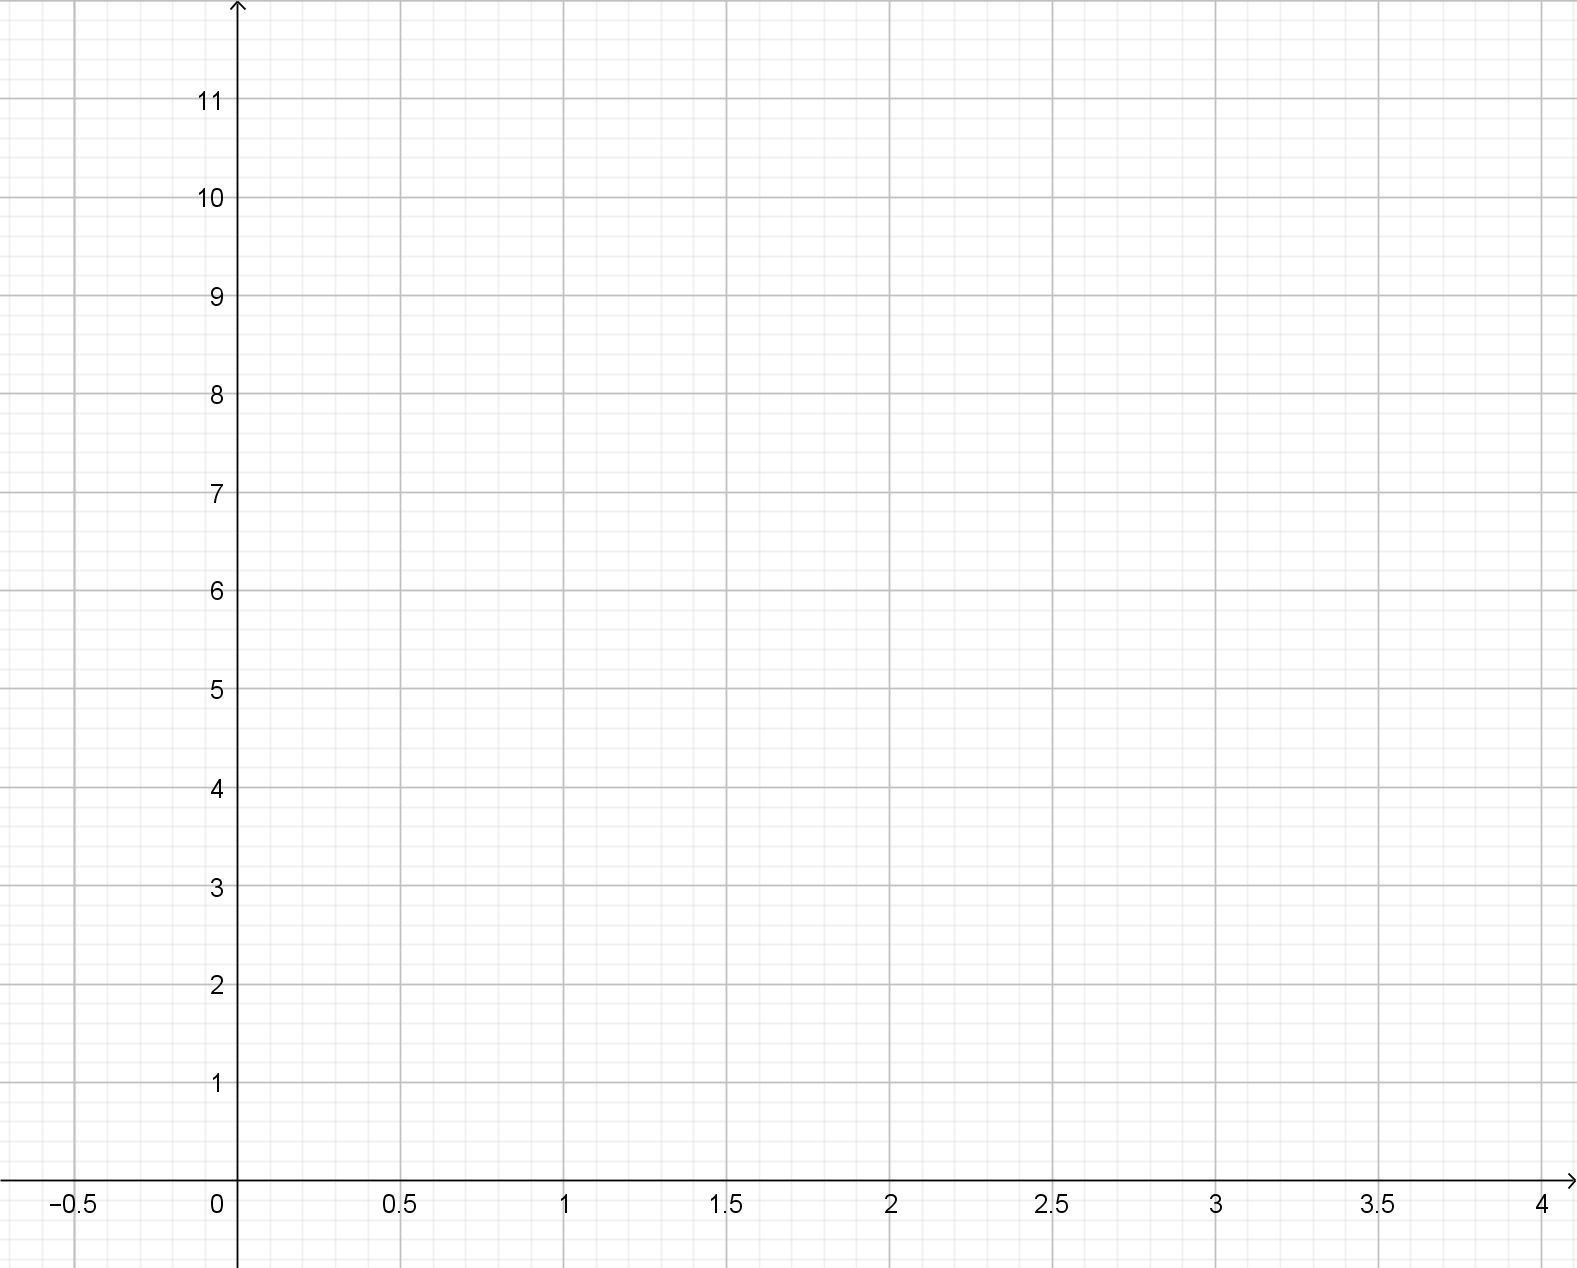
\includegraphics[width=0.4\textwidth,align=t]{HBF/KoordLeer.png} & & 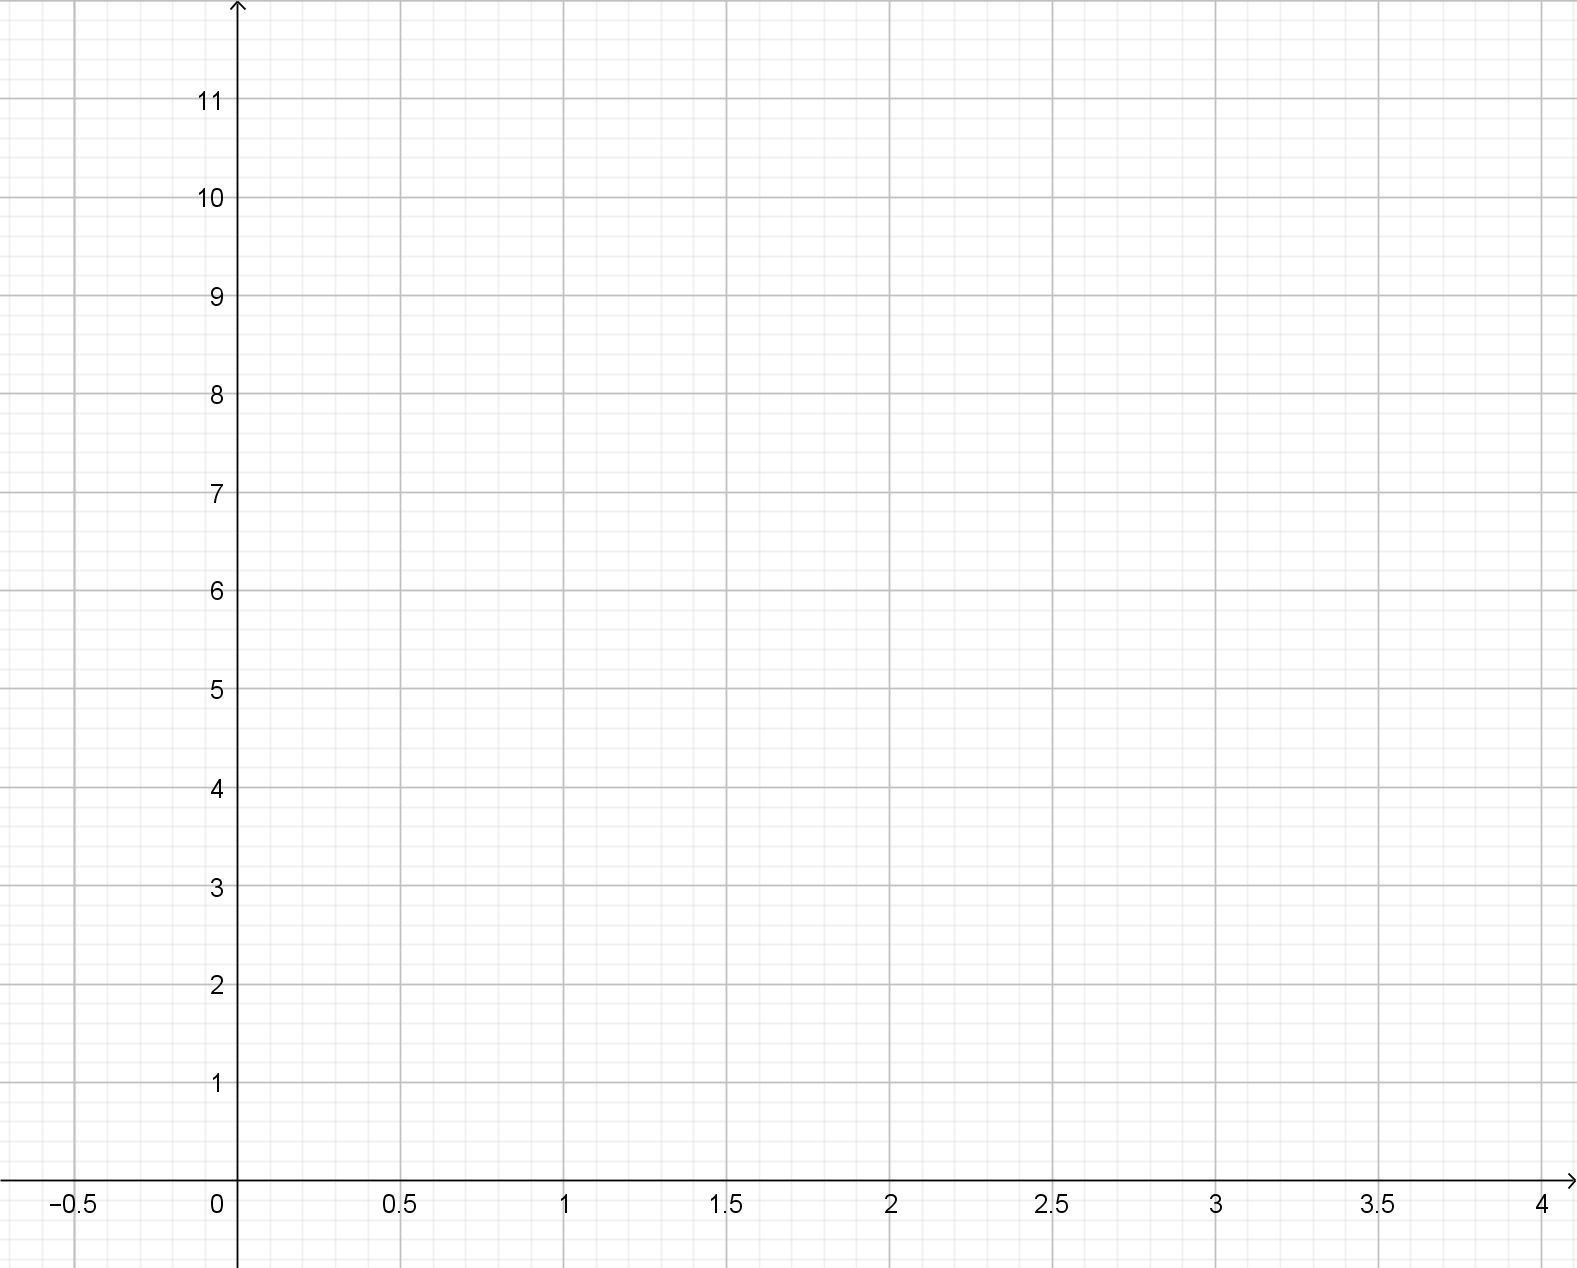
\includegraphics[width=0.4\textwidth,align=t]{HBF/KoordLeer.png}
			\end{tabularx}\\
			\par\noindent
			(c) Berechnen Sie den Schnitt\textbf{punkt} der Gerade aus (a) und (b).\\
		\end{framed}
		\begin{framed}
			\noindent
			\begin{tabularx}{\textwidth}{Xl}\underline{\textbf{Aufgabe 3}}& / 1 + 3 + 1 = \textbf{5 Pkt.}\end{tabularx}\\
			\par\noindent
			Der Vitamin D Gehalt eines Tiefkühl-Fischs entwickelt sich gemäß der mit \(f(x) = 200 -5x\) gegebenen Gleichung. (x: in Wochen, 0 = Zeitpunkt der Tiefkühlung, \(f(x)\): in mg).\\
			\par\noindent
			(a) Berechnen Sie den Vitamin D Gehalt nach einer Tiefkühlung von 10 Wochen.\\
			\par\noindent
			(b) Berechnen Sie die Nullstelle und interpretieren Sie diesen Wert in Bezug auf die Situation.\\
			\par\noindent
			(c) Wenn der Fisch nicht tiefgekühlt gelagert wird, nimmt der Vitamin D Gehalt schneller ab.\\
			Geben Sie eine mögliche Gleichung an, die dies zum Ausdruck bringt!
		\end{framed}
		\begin{framed}
			\noindent
			\begin{tabularx}{\textwidth}{Xl}\underline{\textbf{Aufgabe 4}}& / 2 + 6 + 3 + 3 = \textbf{14 Pkt.}\end{tabularx}\\
			\par\noindent
			Die Leitung eines Seniorenheims stellt fest, dass eine veraltete Waschmaschine hohe Kosten verursacht (sowohl Energie- wie auch Wassertechnisch). Man überlegt daher, eine moderne Waschmaschine gegen eine jährliche Leihgebühr auszuleihen, um so Kosten für Strom und Wasser zu sparen.\\
			Folgende Alternative stehen zur Auswahl:\\
			\par\noindent
			\begin{tabularx}{\textwidth}{|X|X|X|}
				\cline{2-3}
				\multicolumn{1}{l|}{}& \textbf{Alternative 1: veraltete Waschmaschine behalten} & \textbf{Alternative 2: moderne Waschmaschine leihen}\\
				\hline
				\textbf{Kosten für Strom und Wasser pro Waschgang} & \(4,00\)\euro{} & \(2,80\)\euro{}\\
				\hline
				\textbf{Leihgebühr pro Jahr} & - & \(600,00\)\euro{}\\
				\hline
			\end{tabularx}\\
			\par\noindent
			(a) Stellen Sie den Zusammenhang zwischen den Gesamtkosten (\(f(x)\)) und der Anzahl der Waschgänge \((x)\) für beide Alternativen dar!\\
			\par\noindent
			(b) Skizzieren SIe die passenden Geraden für beide Alternativen in das folgende Koordinatensystem und markieren Sie die Anzahl Waschgänge, ab der sich die Neuanschaffung lohnt.\\
			Wählen Sie passende Achsenbeschriftungen!\\
			\par\noindent
			\begin{center}
				\includegraphics[width=0.95\textwidth]{HBF/01_A04b.png}\\
			\end{center}
			\par\noindent
			(c) \underline{\textbf{Berechnen}} Sie die Anzahl der Waschgänge, ab der sich der Abschluss des Leihvertrags lohnt!\\
			\par\noindent
			(d) Ein Wäschereiunternehmen bietet an, für \(3.000\)\euro{} jährlich die gesamte Wäsche zu übernehmen.\\
			\begin{itemize}
				\item[-] Ergänzen Sie die passende Gerade zu dieser Alternativen in das Koordinatensystem aus (b).
				\item[-] Ermitteln sie die erforderliche Anzahl von Waschgängen, damit sich ein Vertragsabschluss \underline{im Vergleich} zur Leihmaschine lohnt!
			\end{itemize}
		\end{framed}
		\begin{framed}
			\noindent
			\begin{tabularx}{\textwidth}{Xl}\underline{\textbf{Aufgabe 5}}& / \textbf{6 Pkt.}\end{tabularx}\\
			\par\noindent
			Der Vorstand eines Sportvereins berät, welche Mitgliedsbeiträge im nächsten Jahr von den Erwachsenen und den Jugendlichen genommen werden soll. Insgesamt benötigt der Verein aus den Mitgliedsbeiträgen einen Erlös von \(40.000\)\euro{}. Der Verein hat 150 erwachsene und 50 jugendliche Mitglieder.\\
			Der Vorsitzende besteht zudem darauf, dass Jugendliche ein Viertel von dem bezahlen, was Erwachsene zahlen.\\
			\par\noindent
			\underline{Ermitteln} Sie die Mitgliedsbeiträge für Jugendliche und Erwachsene!
		\end{framed}
		\begin{center}
			\Large\underline{Viel Erfolg!}
		\end{center}
	\end{test}
\end{document}